\documentclass[12pt,letterpaper]{article}
\usepackage{natbib}

%Packages
\usepackage{pdflscape}
\usepackage{textcomp}
\usepackage{fullpage}
\usepackage{float}
\usepackage{latexsym}
\usepackage{url}
\usepackage{epsfig}
\usepackage{graphicx}
\usepackage{amssymb}
\usepackage{amsmath}
\usepackage{bm}
\usepackage{array}
\usepackage[version=3]{mhchem}
\usepackage{ifthen}
\usepackage{caption}
\usepackage{hyperref}
\usepackage{amsthm}
\usepackage{amstext}
\usepackage{enumerate}
\usepackage[osf]{mathpazo}
\usepackage{dcolumn}
\usepackage{lineno}
\usepackage{dcolumn}
\newcolumntype{d}[1]{D{.}{.}{#1}}

\pagenumbering{arabic}


%Pagination style and stuff
\linespread{2}
\raggedright
\setlength{\parindent}{0.5in}
\setcounter{secnumdepth}{0} 
\renewcommand{\section}[1]{%
\bigskip
\begin{center}
\begin{Large}
\normalfont\scshape #1
\medskip
\end{Large}
\end{center}}
\renewcommand{\subsection}[1]{%
\bigskip
\begin{center}
\begin{large}
\normalfont\itshape #1
\end{large}
\end{center}}
\renewcommand{\subsubsection}[1]{%
\vspace{2ex}
\noindent
\textit{#1.}---}
\renewcommand{\tableofcontents}{}
%\bibpunct{(}{)}{;}{a}{}{,}

%---------------------------------------------
%
%       START
%
%---------------------------------------------

\begin{document}

%Running head
\begin{flushright}
Version dated: \today
\end{flushright}
\bigskip
\noindent RH: disparate views on disparity.

\bigskip
\medskip
\begin{center}

\noindent{\Large \bf Disparate views on disparity.} 
\bigskip

\noindent {\normalsize \sc Thomas Guillerme$^1$$^,$$^*$, Natalie Cooper$^2$, Philip Donoghue$^3$}\\
\noindent {\small \it 
$^1$Imperial College London, Silwood Park Campus, Department of Life Sciences, Buckhurst Road, Ascot SL5 7PY, United Kingdom.\\}
\end{center}
\medskip
\noindent{*\bf Corresponding author.} \textit{guillert@tcd.ie}\\  
\vspace{1in}

%Line numbering
\modulolinenumbers[1]
\linenumbers

%---------------------------------------------
%
%       ABSTRACT
%
%---------------------------------------------

\newpage
\begin{abstract}

\begin{enumerate}
    blablalbalba
\end{enumerate}

\end{abstract}

\noindent (Keywords: disparity)\\

\vspace{1.5in}

\newpage 

%---------------------------------------------
%
%       INTRODUCTION
%
%---------------------------------------------

\section{Introduction}

Disparity, as a concept or set of toolkits is used a lot in biology and is more and more used every year.

\begin{figure}[!htbp]
\centering
   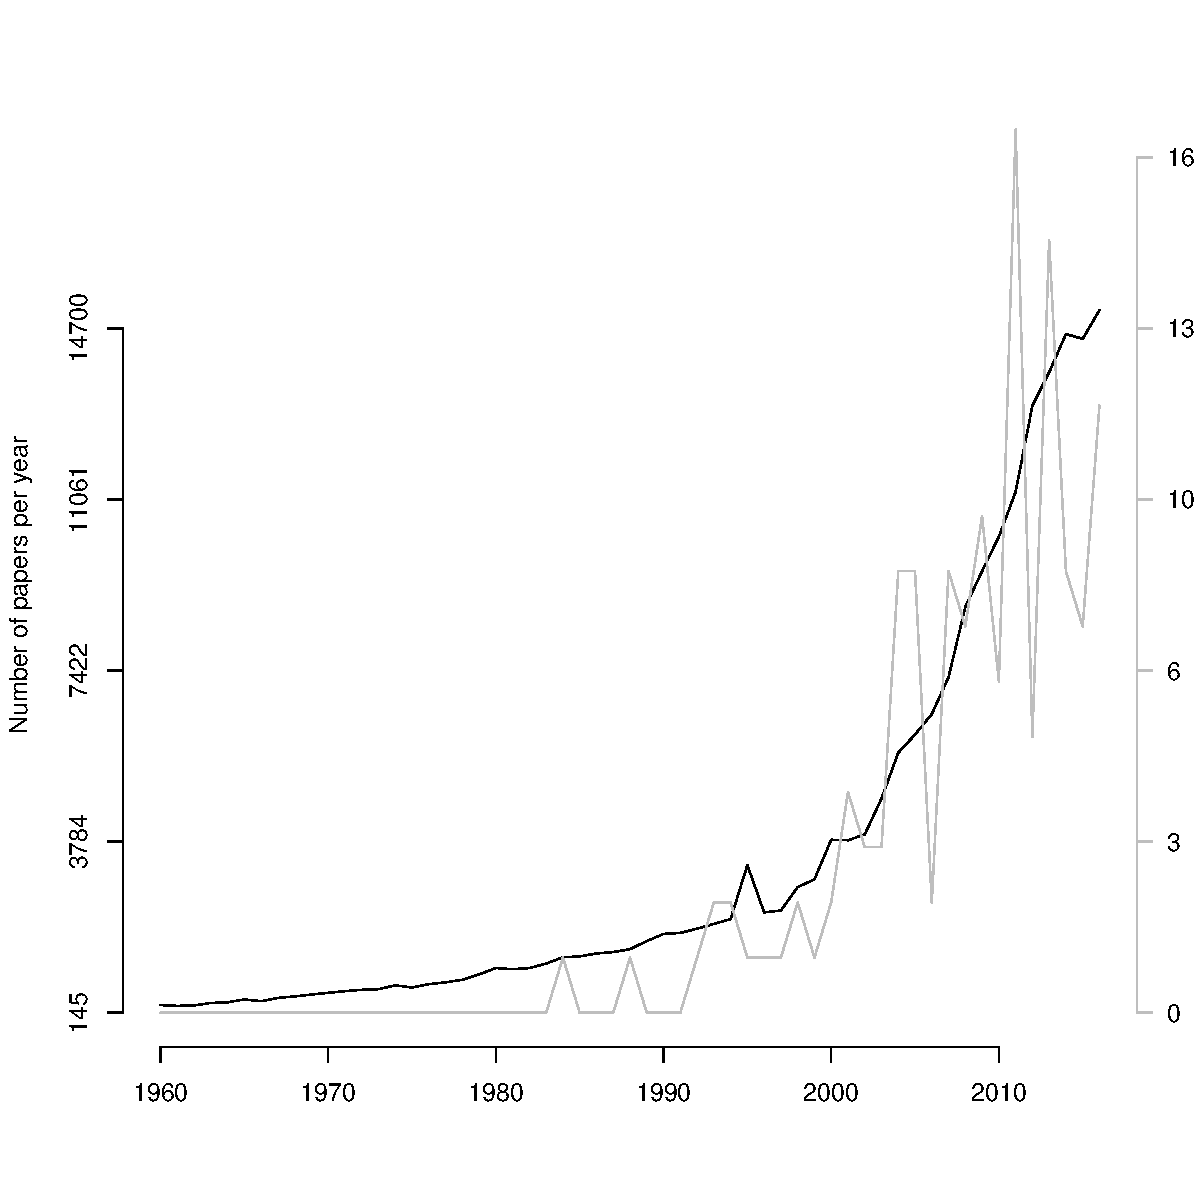
\includegraphics[width=1\textwidth]{Figures/GoogleScholarOccurences.pdf} 
\caption{Number of papers on Google Scholar matching the search ``morphological disparity'' per year. In black, the match is in the paper and in grey, in the title.}
\label{Fig:GoogleOccurences}
\end{figure}

In most of these papers, they trace back the disparity concept to seminal papers from the 90s: \cite{gould1989wonderful,gould1991disparity,briggs1992morphological,Wills1994,Foote01071994,Foote29111996,jernvall1996molar,foote1997evolution}.
However, being such a broad and obvious concept, it can probably be stretched back to way earlier.

\cite{prentice2011} define disparity as: ``a term widely (albeit not always consistently) used to describe the range of forms in a group of organisms, or the difference among different body plans''.




Biological data are complex; understanding the ecology and evolution of species often requires that we analyse multiple variables that covary with each other, and through space and time.
One solution to this problem is to analyse data in a multivariate framework.
Multivariate analyses aim to capture and incorporate this multidimensional complexity, while providing outputs that are interpretable in a physical world of only three dimensions.
Classical multidimensional species features that have been analysed through multivariate data ranges from their morphology \citep{raup1966geometric}, to their functional traits \citep{diaz2016global}.
However, such analysis are not limited at the species level and can also be applied to ecosystems \citep{DonohueDim}.

Key multidimensional features of species that have important roles in ecology and evolution include morphology, functional traits. etc. etc.
Many of these can be represented as matrices, these can be used in our package.
In the interests of clarity/brievety, we here focus on just one kind of data: morphological diversity.


Furthermore, we will also make a clear distinction between the multidimensional space which is a specific mathematical object and the disparity, which is a metric describing or summarising one or more aspects of this space.


Both can be defined in various ways depending on the authors, for example, disparity is defined as the weighted mean pairwise dissimilarity in \cite{Close2015} or the ellipsoid volume in \cite{DonohueDim} and the multidimensional space is defined as the morphospace in \cite{raup1966geometric} and the morpho-functional space in \cite{diaz2016global}.




The multidimensional space can be defined in many ways and arise from many mathematical transformations of the data such as the pairwise distance matrix \citep{Close2015}, a principal coordinates analysis \citep[PCO;][]{Brusatte12092008}, a principal components analysis \citep[PCA;][]{zelditch2012geometric}, a multidimensional scaling \citep[MDS;][]{DonohueDim}, etc.
Similarly, disparity metrics \citep[or indices;][]{Hopkins2017} can defined in many ways \citep[e.g.][or combinations thereof]{Wills2001,Ciampaglio2001,foth2012different,DonohueDim,Hughes20082013,finlay2015morphological,Close2015,diaz2016global}.
Finally, difference between disparity metrics can also be measured in many ways: using NPMANOVA \citep[e.g.][]{Brusatte12092008}, multidimensional permutation test \citep[e.g.][]{diaz2016global} or even simple confidence interval overlap \citep[e.g.][]{halliday2016eutherian}.

This variety of definitions and analysis have been developed in an equal variety of softwares such as \texttt{GINGKO} in javascript \citep{bouxin2005ginkgo,de2007ginkgo} or \texttt{geomorph} \citep{adams2013geomorph,adams2017geometric}, \texttt{Claddis} \citep{Claddis}, or \texttt{vegan} \citep{oksanen2007vegan} in R \citep{R}.
This results in the need to learn different languages (or at least - when restricted to R - different packages with different standards) as well as making analysis sometimes idiosyncratic and often complex to repeat since they are based on a particular feature from a particular software.
For example, in the excellent and widely used \texttt{geomorph} package morphological disparity analysis can be ran using the \texttt{morphol.disparity} function.
Unfortunately, however, the multidimensional space can only be defined as the ordination of the procrustes transform of geometric morphometric landmarks, the disparity can only be defined as the Procrustes variance and the difference between groups can only be measured through permutation tests \citep{zelditch2012geometric,adams2013geomorph,adams2017geometric}.




Disparity is an old concept blabalbal

\section{What \textit{is} disparity}

From a semantic view: morphospace or aspect of the morphospace?

From a biological view: what does an increase or a decrease in disparity represent?

\section{Why do we need disparity}

What are the fundamental questions we should use to answer disparity questions?

What are the questions we should not answer with disparity?

\section{What is missing}

Methods?
Data?

\section{Conclusion}

Yay!

% \section{Data availability and reproducibility}
% Data are available on Dryad or Figshare.
% Code for reproducing the analyses is available on GitHub (\url{github.com/TGuillerme/SpatioTemporal_Disparity}).

\section{Acknowledgments}
Royal Society..
I acknowledge support from European Research Council under the European Union's Seventh Framework Programme (FP/2007 – 2013)/ERC Grant Agreement number 311092 awarded to Martin D. Brazeau.


\bibliographystyle{sysbio}
\bibliography{References}

\end{document}
